%---------------------------------------------------------------------------%
\lecture{Research Presentation}{lec_present_result}
%---------------------------------------------------------------------------%
\section{Properties of Equilibria}

%---------------------------------------------------------------------------%

\begin{frame}[fragile]
    \frametitle{Marginally Stable Thermal Equilibria (MSTE)}
    % \vspace{-0.2cm}
    % \begin{itemize}

    %     \item Initial $=$ initial condition of quasilinear model (we used $\tanh$ functions)
        
    %     \item ECS $=$ Exact Coherent States -- steady solutions to the nonlinear problem
         
    %     \item MSTE $=$ equilibrated quasilinear solutions
        
    %     \item DNS $=$ temporaly-averaged Direct Numerical Simulations of the nonlinear problem
        

    % \end{itemize}
    % \vfill\vfill\vfill\vfill\vfill\vfill\vfill
    % $\quad$ *Note the prominent dips in the 
    
    % $\quad\;\,$ MSTE near the boundaries
    % \vfill\vfill\vfill\vfill\vfill\vfill\vfill\vfill
    % \tikzart[t=p,x=0,y=-2.5,w=6]{flow}
    % \begin{figure}
    \begin{center}
        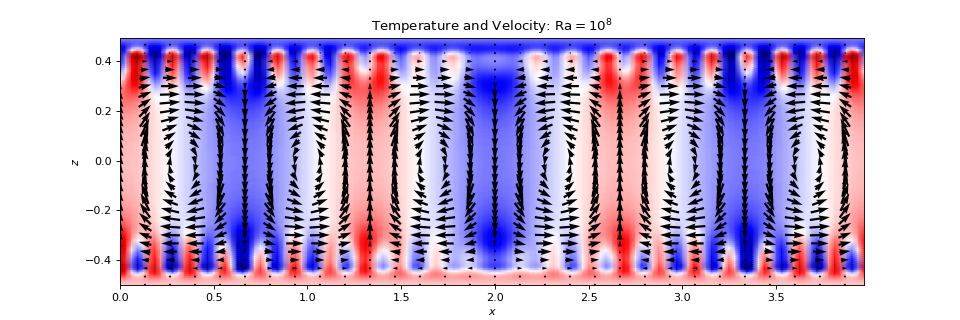
\includegraphics[width=15cm]{flow1.png}
    \end{center}
    % \end{figure}
\end{frame}


% \begin{frame}[fragile]
%     \frametitle{MSTE $\overline{T}$ Profiles}
%     \vspace{-0.2cm}
%     \begin{itemize}

%         \item Initial $=$ initial condition of quasilinear model (we used $\tanh$ functions)
        
%         \item ECS $=$ Exact Coherent States -- steady solutions to the nonlinear problem
         
%         \item MSTE $=$ equilibrated quasilinear solutions
        
%         \item DNS $=$ temporaly-averaged Direct Numerical Simulations of the nonlinear problem
        

%     \end{itemize}
%     \vfill\vfill\vfill\vfill\vfill\vfill\vfill
%     $\quad$ *Note the prominent dips in the
    
%     $\quad\;\,$ MSTE near the boundaries
%     \vfill\vfill\vfill\vfill\vfill\vfill\vfill\vfill
%     \tikzart[t=p,x=1,y=-2.5,w=6]{T_profs_na}
% \end{frame}

\begin{frame}[fragile]
    \frametitle{MSTE Flux and Spectra}
    \begin{columns}
        \begin{column}{.28\textwidth}
            \begin{itemize}
                \item High-$\rm{Ra}$ cases have additional marginal modes at higher wavenumbers\newline
                
                \item High wavenumber advections are concentrated near the boundaries, combating the diffusion of their thin boundary layers
            \end{itemize}
        \end{column}
        \begin{column}{.28\textwidth}
            \centering
            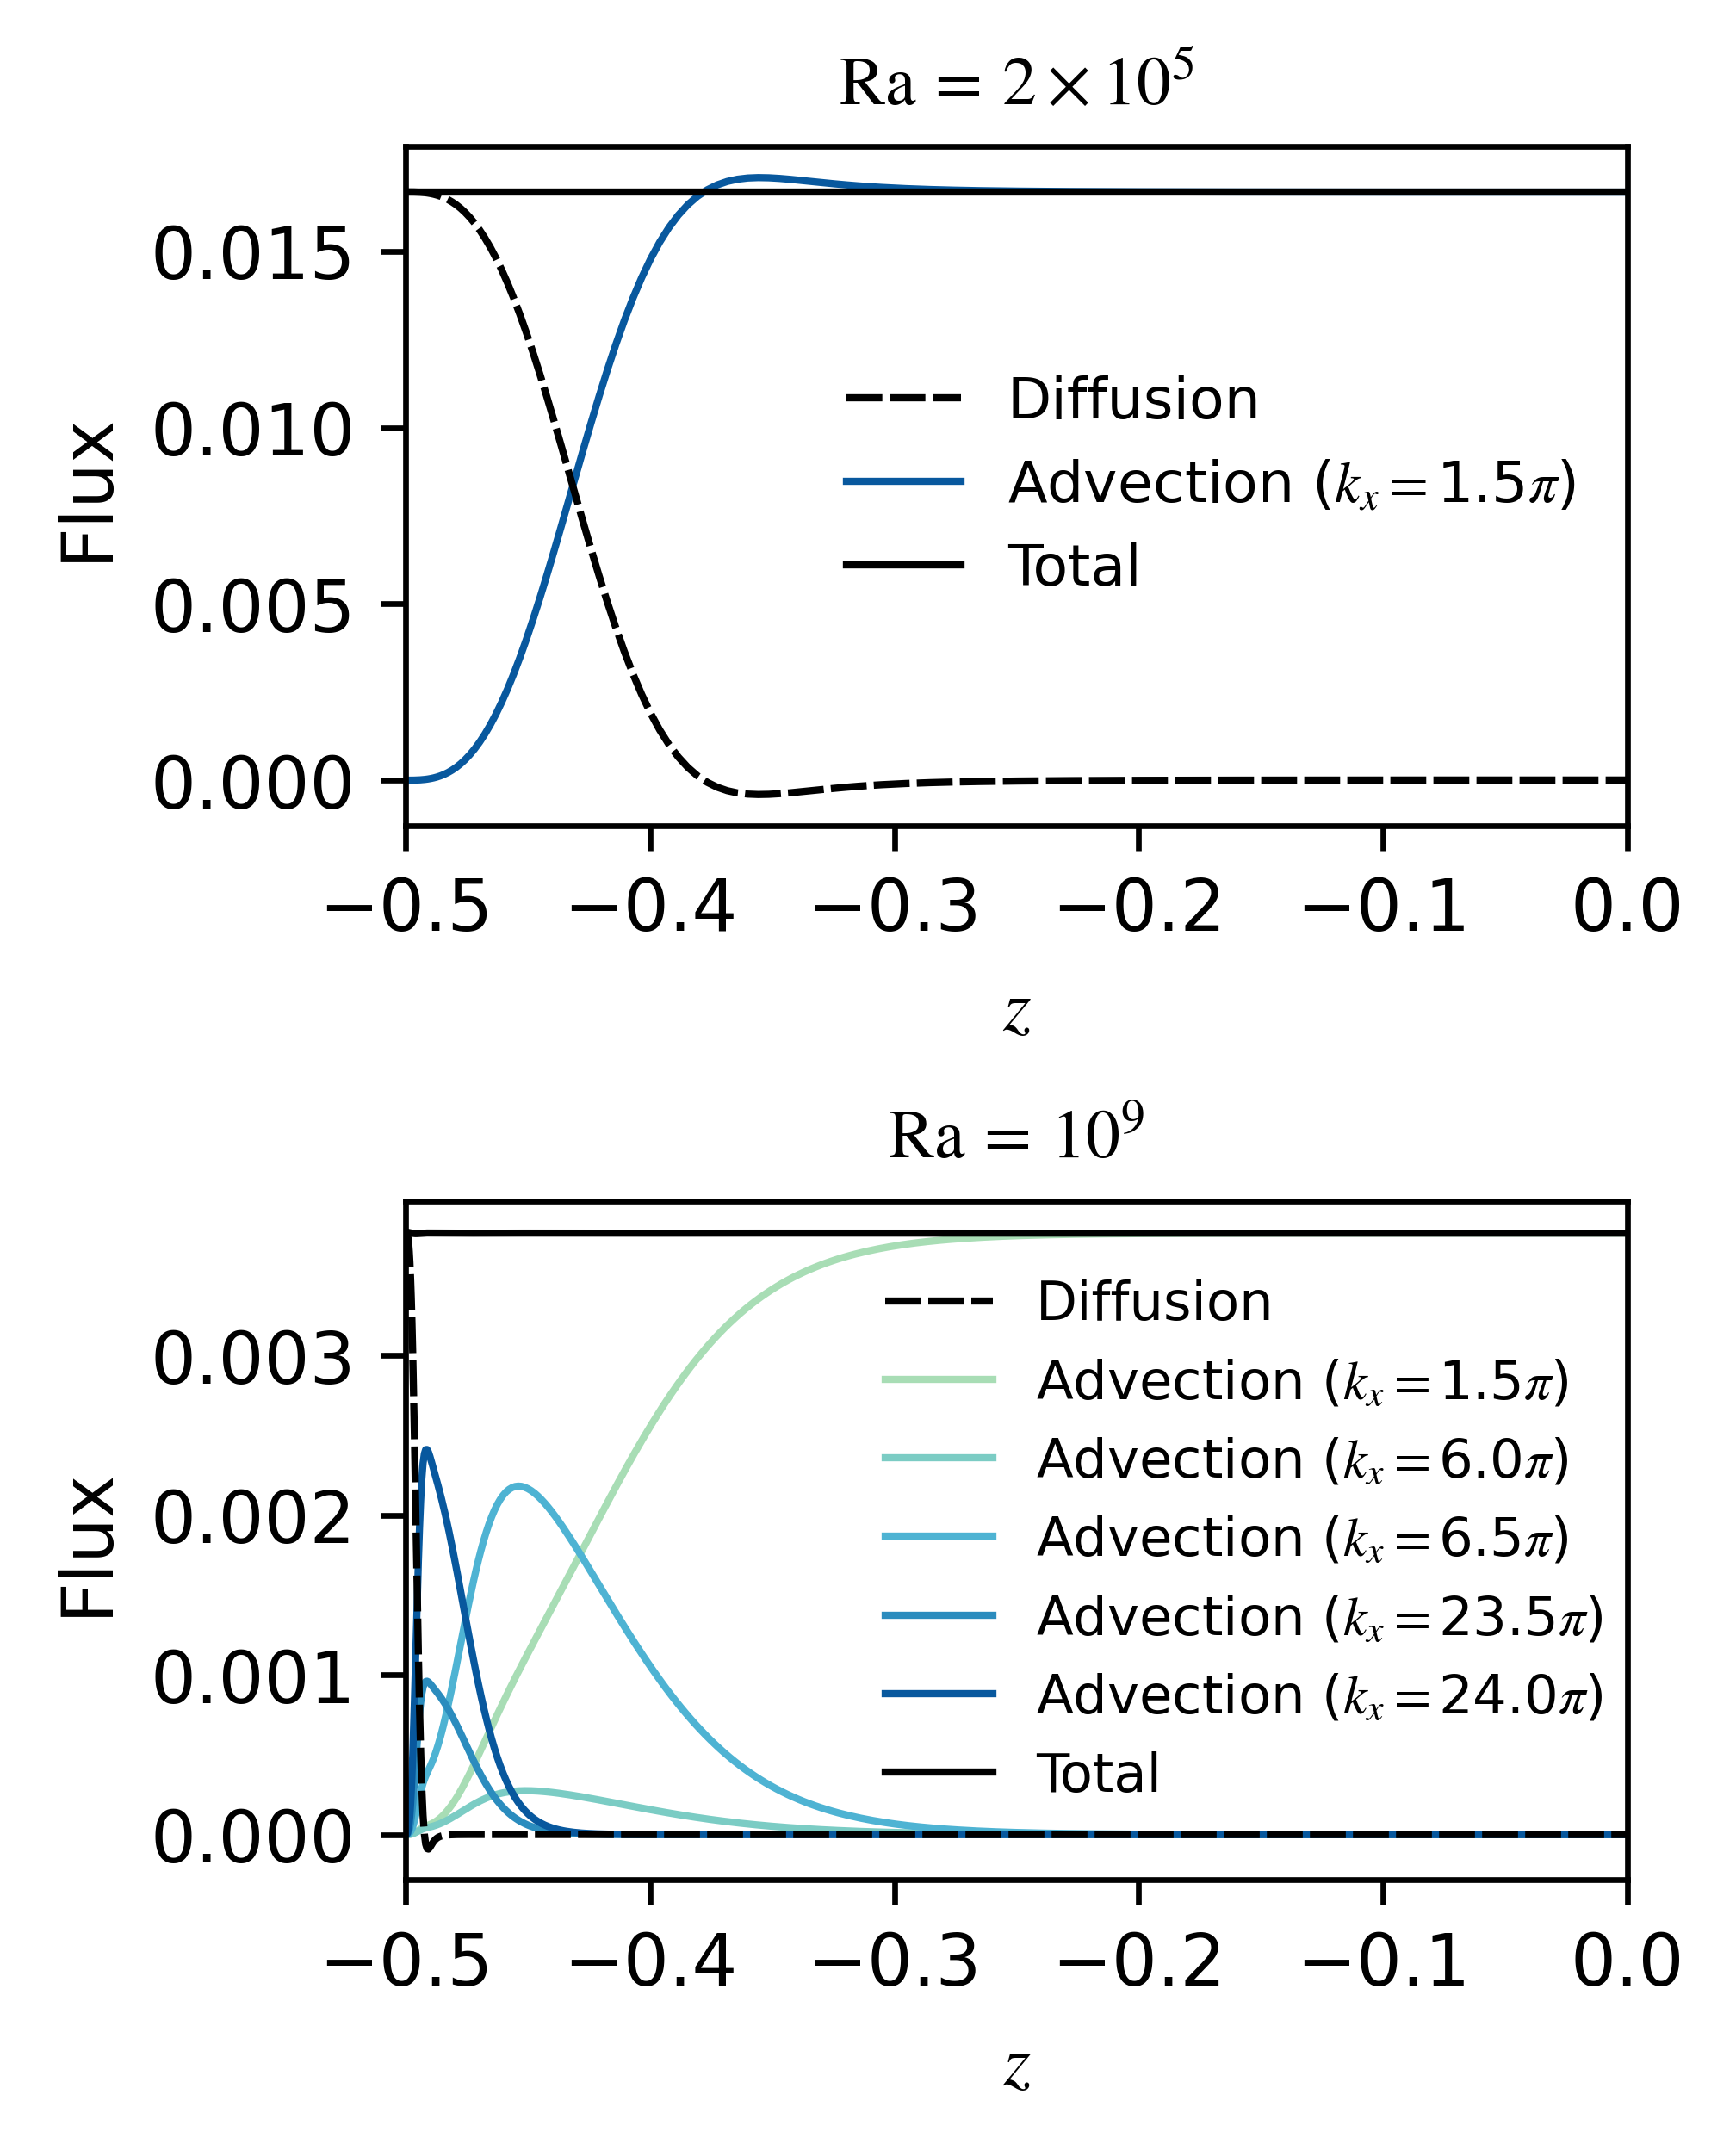
\includegraphics[height=1.4\textwidth]{flux_sup_n}
            {Flux}
        \end{column}
        \begin{column}{.28\textwidth}
            \centering
            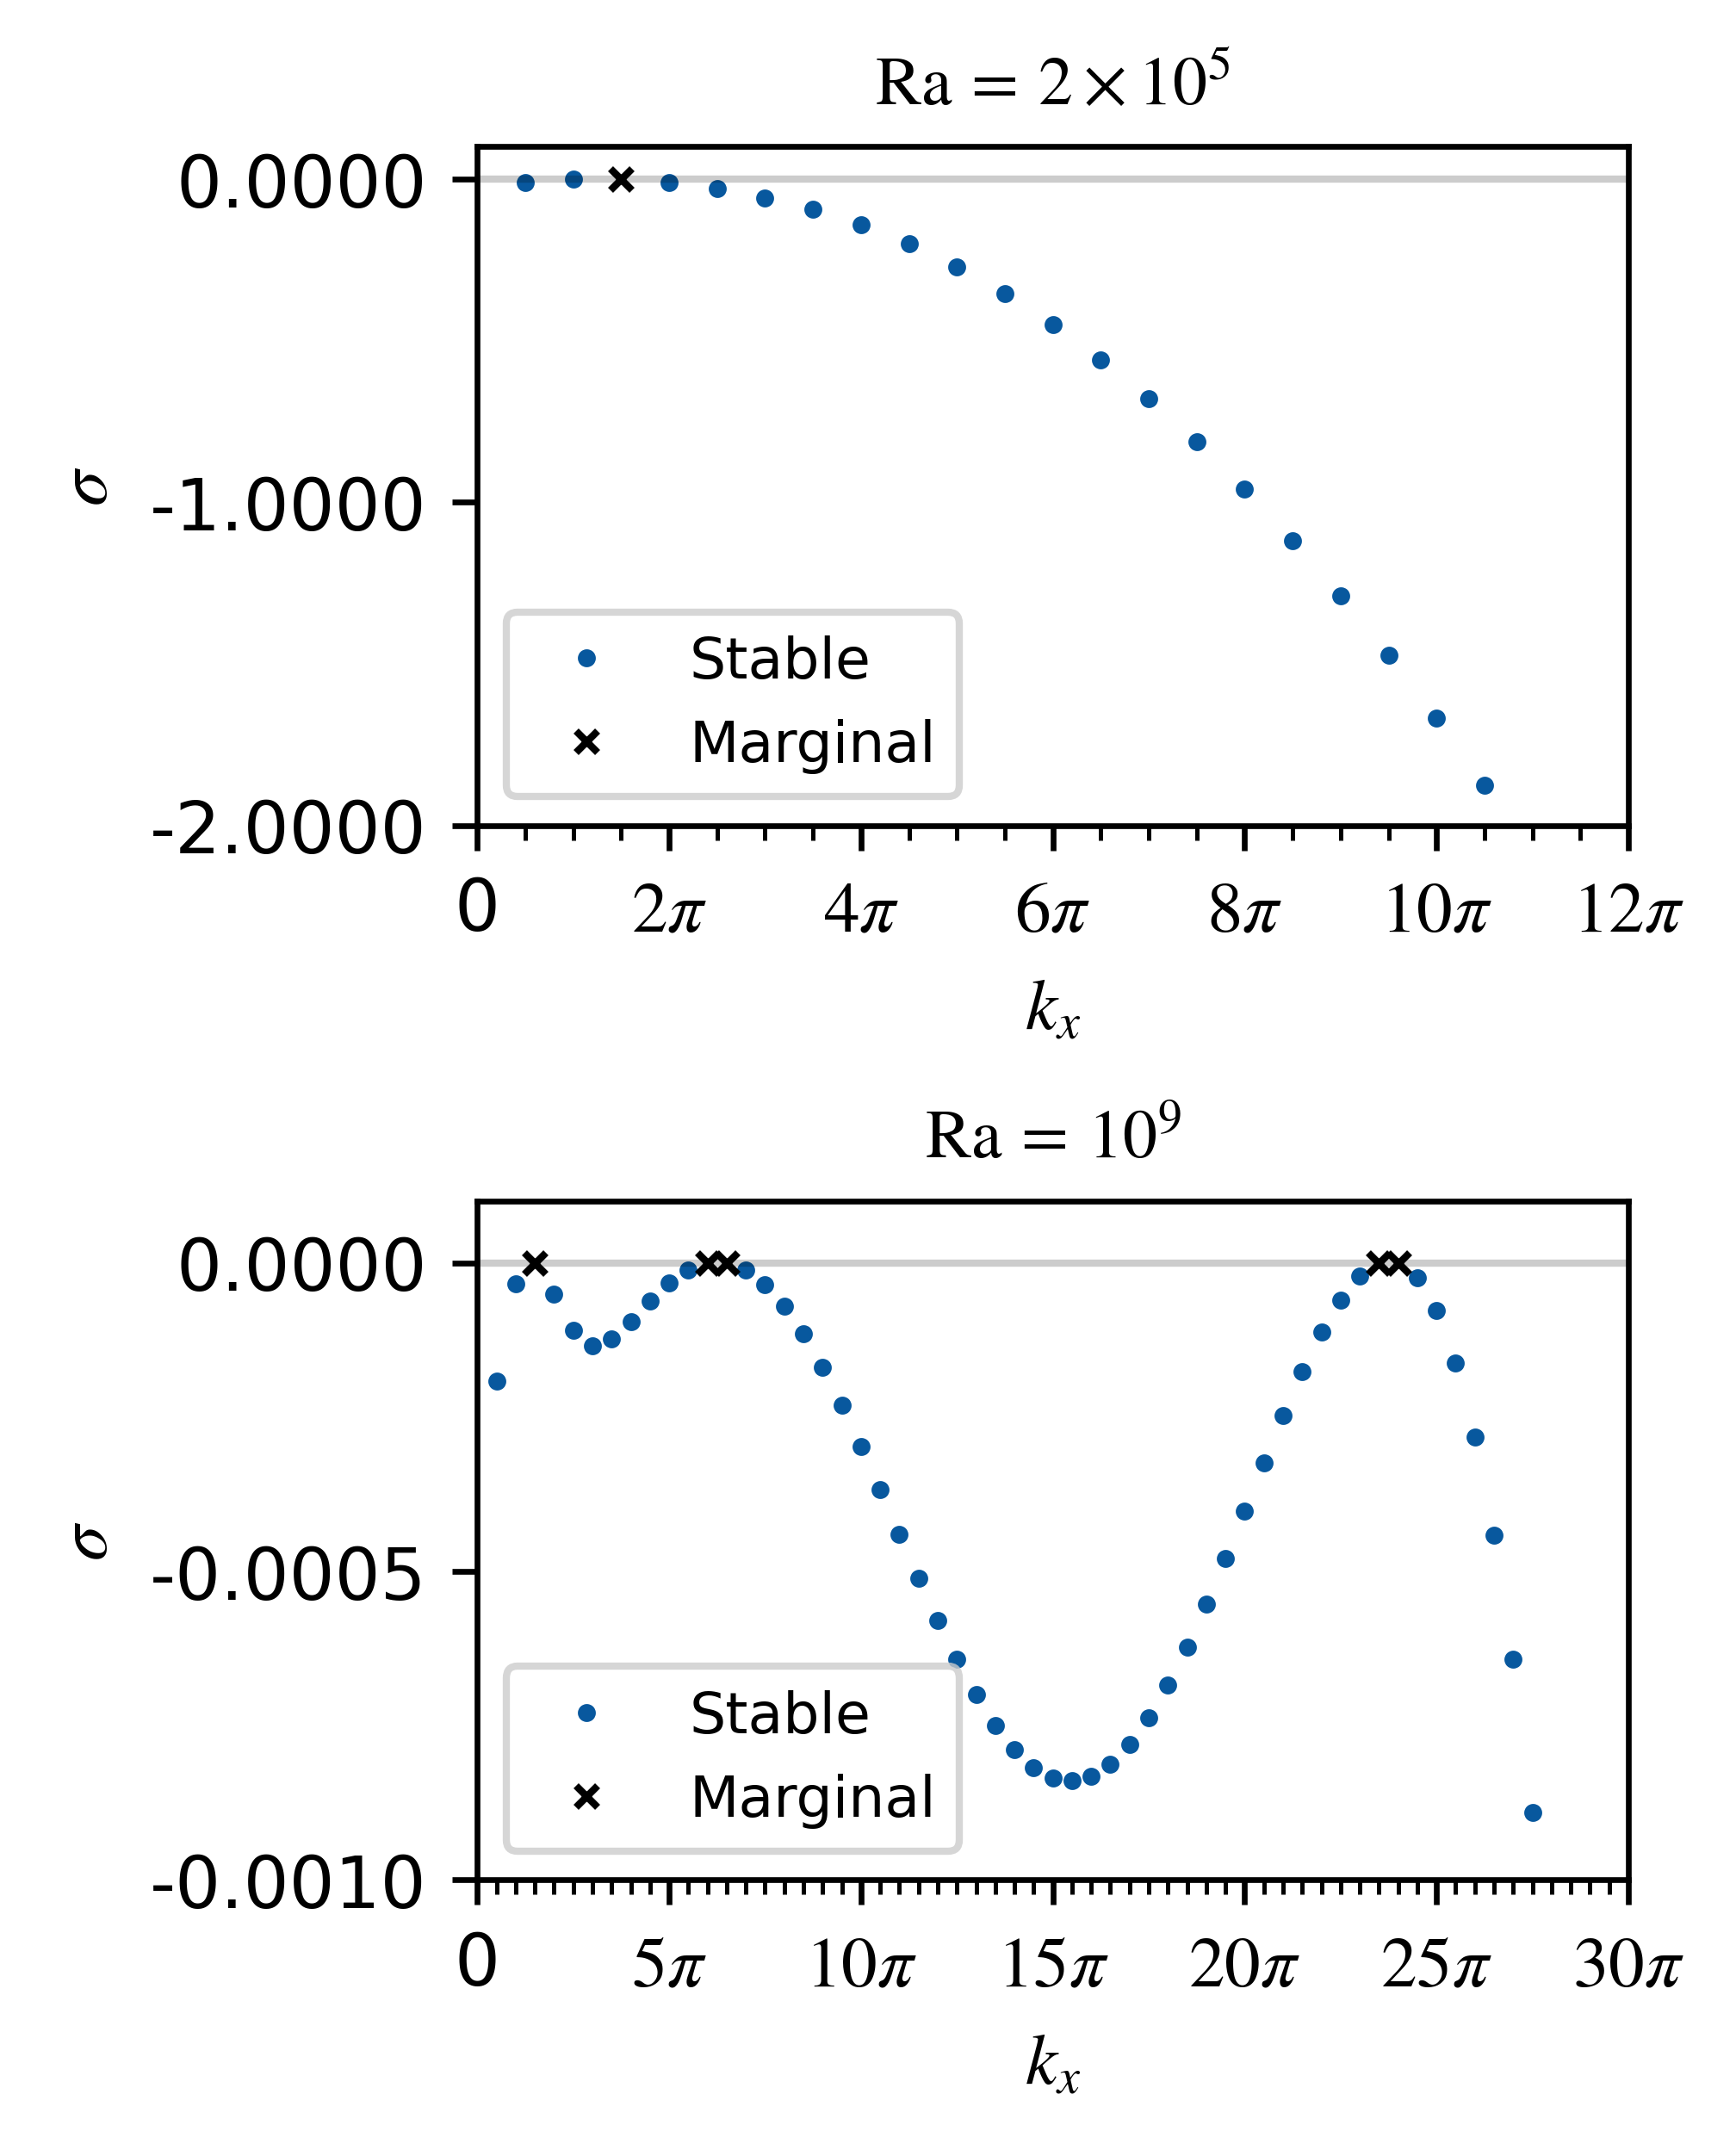
\includegraphics[height=1.4\textwidth]{EV_spectra_2ra}
            {Spectra}
        \end{column}
    \end{columns}
\end{frame}

% \begin{frame}[fragile]
%     \frametitle{MSTE Marginal Wavenumbers}
%     \begin{columns}
%         \begin{column}{.4\textwidth}
%             \begin{itemize}
%                 \item Branches are color-coded according to their proximities to local maxima

%                 \item The $k_x = \frac{3\pi}{2}$ mode is present $\forall \rm{Ra}$. This mode forms the familiar large-scale convective structure
                
%                 \item $k_x > \frac{3\pi}{2}$ modes' wavenumbers obey power laws
%             \end{itemize}
%         \end{column}
%         \begin{column}{0.6\textwidth}
%             \centering
%             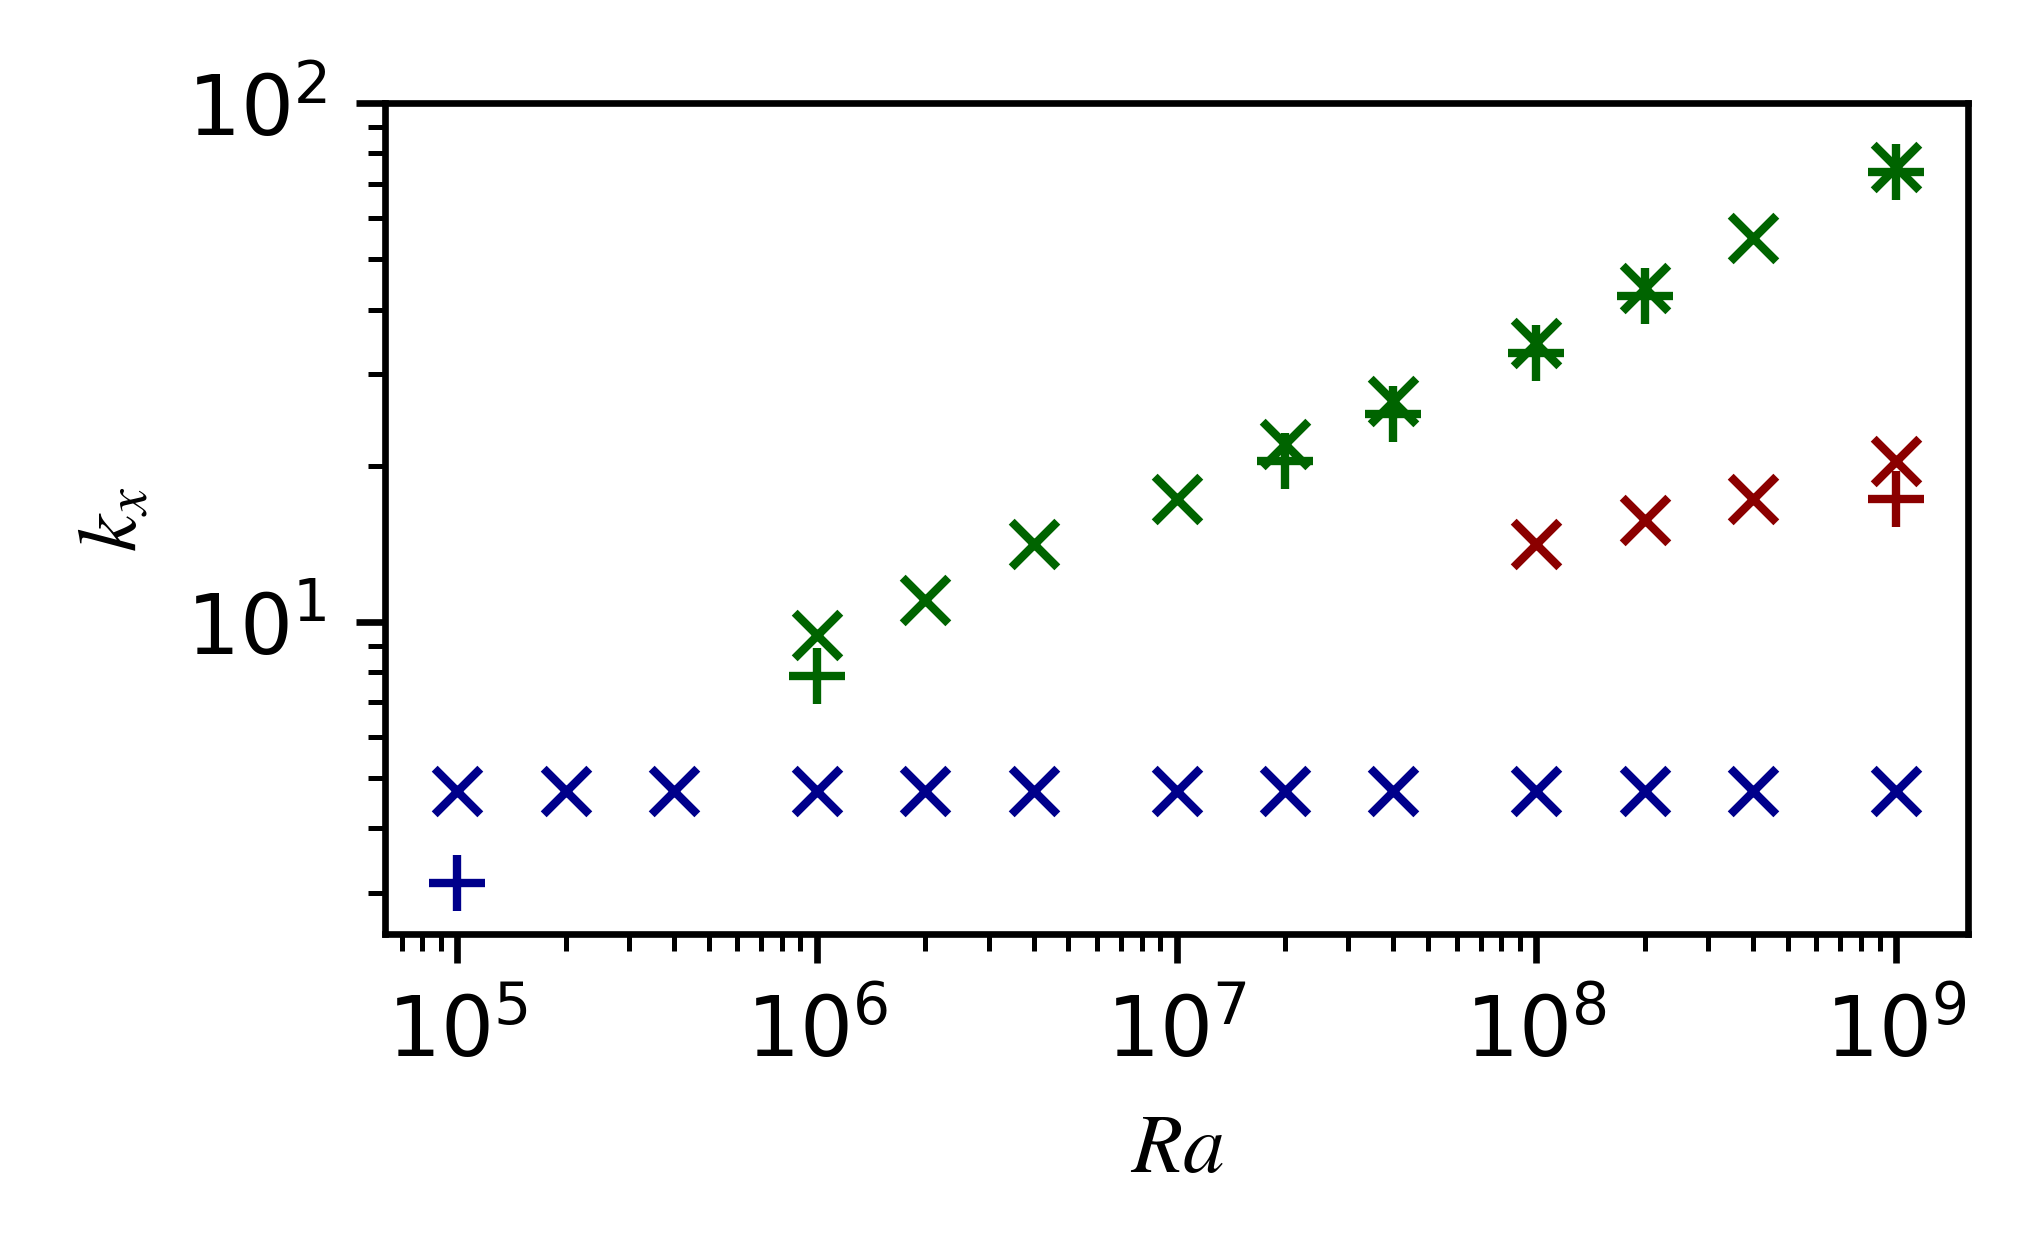
\includegraphics[width=0.9\textwidth]{kx_m_ra1}
%             {Wavenumbers $k_x$ of marginally-stable MSTE modes}
%         \end{column}
%     \end{columns}
% \end{frame}

% \begin{frame}[fragile]
%     \frametitle{MSTE Boundary Layer Thicknesses $\delta$}
%     \begin{columns}
%         \begin{column}{.4\textwidth}
%             \begin{itemize}

%                 \item We define $\delta$ as the distance from the boundary where $\partial_z \overline{T}=0$\newline
                

%                 \item For $\rm{Ra} \geq 10^6$, the maximum wavenumbers scale with $\delta^{-1}$\newline

%                 \item $\delta$ provides a minimum $z$-length scale for MSTE $\overline{T}$ profiles

%             \end{itemize}
%         \end{column}
%         \begin{column}{0.6\textwidth}
%             \centering{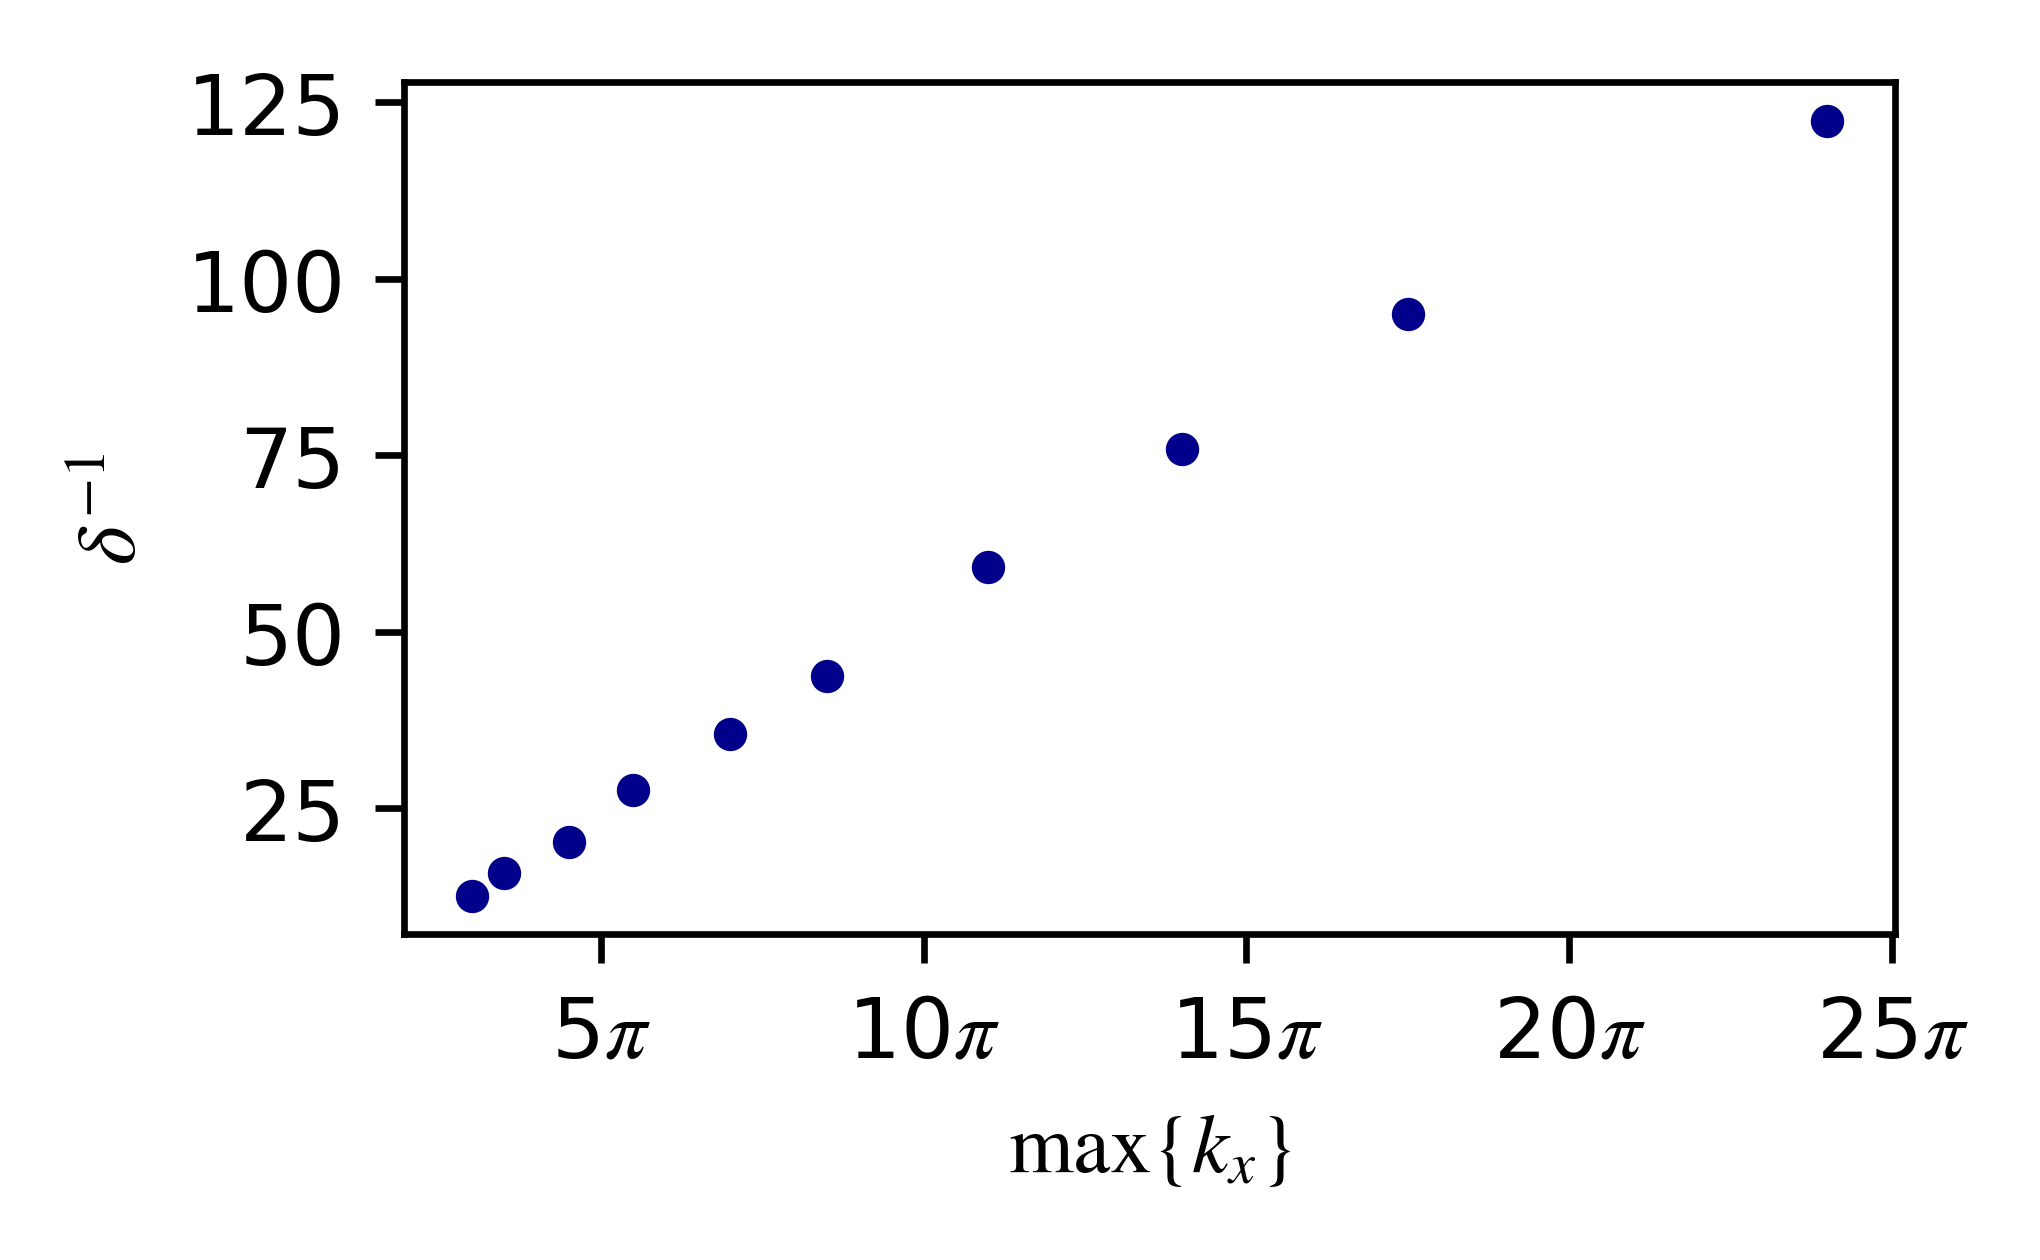
\includegraphics[width=0.9\textwidth]{del_kx_inv}}
            
%             {$\delta \;=$  boundary layer thickness of $\overline{T}$
            
%             ($\rm{Ra} \geq 10^6$)
%             }
%         \end{column}
%     \end{columns}
% \end{frame}

\begin{frame}[fragile]
    \frametitle{Self-Similarity in $\overline{T}$ Near Boundaries}
    \begin{columns}[T]
        \begin{column}{0.5\textwidth}
            \centering{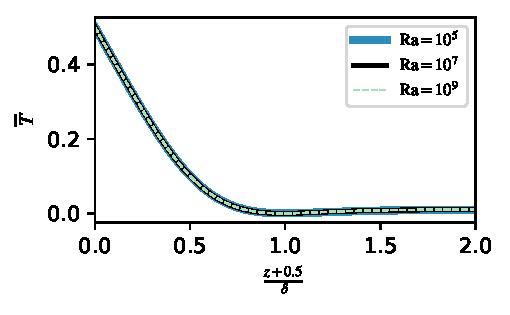
\includegraphics[height=0.7\textwidth]{b0_delta_solid}}
            
            {Rescaling according to $\delta$ reveals self-similarity in $\overline{T}$ profiles}
        \end{column}
        \begin{column}{0.5\textwidth}
            % \vspace{-1cm}
            \vfill
            \centering{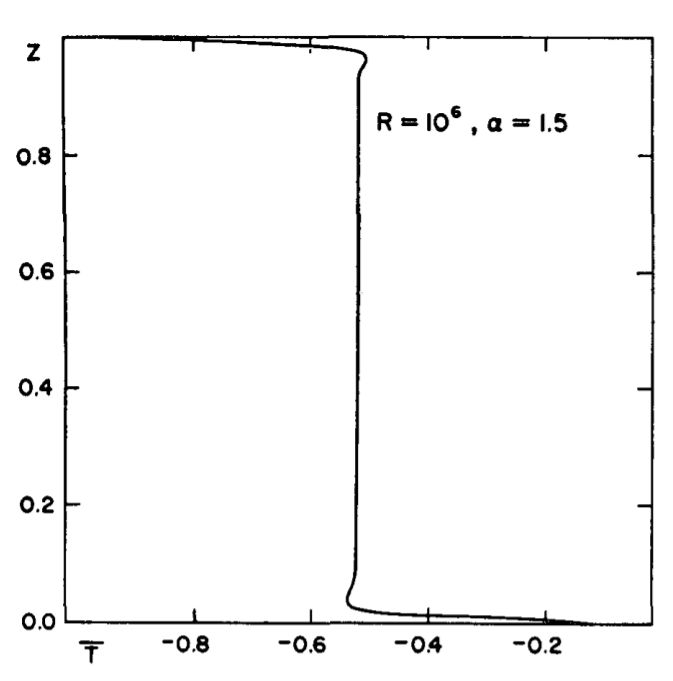
\includegraphics[height=0.75\textwidth]{herring}}
            \vfill
            \vfill
            
            {(Herring 1963)}
            \vfill
            \vfill
            \vfill
        \end{column}
    \end{columns}
\end{frame}
%---------------------------------------------------------------------------%

\begin{frame}[fragile]
    \frametitle{MSTE Nusselt Numbers: Classical Scaling}
    \begin{itemize}
        \item MSTE exhibit ``classical'' or ``Malkus'' scaling: $\delta \sim \rm{Nu} \sim \rm{Ra}^{1/3}$

        \item MSTE transport heat more efficiently than simulations (DNS) and steady nonlinear solutions (ECS)\newline
        

        \centering
        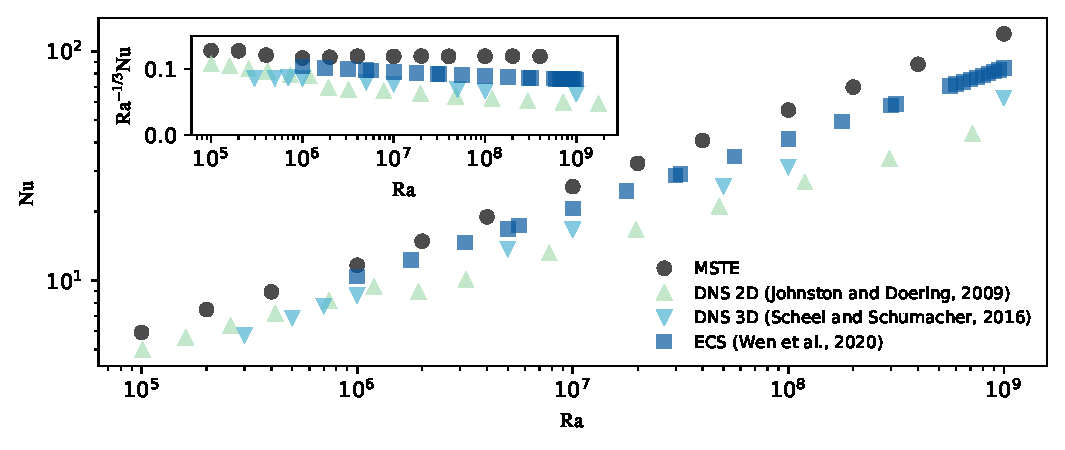
\includegraphics[width=0.7\textwidth]{nu_ra}

    \end{itemize}
\end{frame}
%---------------------------------------------------------------------------%
